% \date{May 14, 2024}
% \author{Deralive}
% \title{华东师范大学软件学院实验报告模板}
% 注意事项:编译两次,以确保目录、页码完整显示
\def\allfiles{}

%————————————多文件编译————————————%
% \ifx\allfiles\undefined
% 	    \begin{document}
% \else
% \fi

% Content

% \ifx\allfiles\undefined
% 	    \end{document}
% 	\else
% 	\fi
%—————————————————————————————————%

\documentclass[14pt,a4paper,UTF8,twoside]{article}

\usepackage[paperwidth=210mm, paperheight=297mm, margin=2cm]{geometry}
\usepackage[utf8]{inputenc}
\usepackage{ctex}

% Formatting Packages ——————————————————————————————————————
\usepackage{multicol}
\usepackage{multirow}
\usepackage{enumitem}
\usepackage{indentfirst}
\usepackage[toc]{multitoc}

% Math & Physics Packages ————————————————————————————
\usepackage{amsmath, amsthm, amsfonts, amssymb}
\usepackage{amssymb}
\usepackage{setspace}
\usepackage{physics}
\usepackage{cancel}
\usepackage{nicefrac}

% Image-related Packages —————————————————————————————
\usepackage{graphics, graphicx}
\usepackage{tikz}
\usetikzlibrary{arrows.meta}
\usepackage{pgfplots}
\pgfplotsset{compat=1.18}
\usepackage{xcolor}
\usepackage{fourier-orns}
\usepackage{lipsum}


%% Silakan otak-atik judul di sini
\title{\texorpdfstring{\vspace{-1.5em}}{}\textbf{概率论与数理统计}}
\author{张梓卫 10235101526}
\date{\the\day \ \monthyear}

% Kalau mau bab pertama nomornya 0, ganti 0 jadi -1
\setcounter{section}{0}

\renewcommand*\contentsname{第十三周概率论作业}
\renewcommand*{\multicolumntoc}{2}
\setlength{\columnseprule}{0.5pt}

% Layouting Packages ————————————————————————————————————————
\usepackage{titlesec}
\usepackage{fancyhdr}
\pagestyle{fancy}
\setlength{\headheight}{14.39996pt}
\fancyfoot[C]{\textit{By Deralive (10235101526)}}
\fancyfoot[R]{\thepage}

\fancyhead[LE, RO]{\textsl{\rightmark}}
\fancyhead[LO, RE]{\textsl{\leftmark}}

\renewcommand\headrule{
	\vspace{-6pt}
	\hrulefill
	\raisebox{-2.1pt}
	{\quad\floweroneleft\decoone\floweroneright\quad}
	\hrulefill}

\renewcommand\footrule{
	\hrulefill
	\raisebox{-2.1pt}
	{\quad\floweroneleft\decoone\floweroneright\quad}
	\hrulefill}
  
\newcommand{\fpb}[2]{\mathrm{FPB}(#1, #2)}
\newcommand{\kpk}[2]{\mathrm{KPK}(#1, #2)}

% Reference and Bibliography Packages ————————————————————
\usepackage{hyperref}
\hypersetup{
    colorlinks=true,
    linkcolor={black},
    citecolor={biru!70!black},
    urlcolor={biru!80!black}
}

\numberwithin{equation}{section}

% Silakan lihat dokumentasi package biblatex
% untuk format sitasi yang diperlukan
\usepackage[backend=biber]{biblatex}
\addbibresource{ref.bib}
\makeatletter
\def\@biblabel#1{}
\makeatother

\renewcommand{\mod}{\mathrm{mod} \ }

% Titling
\newcommand{\garis} [3] []{
	\begin{center}
		\begin{tikzpicture}
			\draw[#2-#3, ultra thick, #1] (0,0) to (1\linewidth,0);
		\end{tikzpicture}
	\end{center}
}

\newcommand{\monthyear}{
  \ifcase\month\or January\or February\or March\or April\or May\or June\or
  July\or August\or September\or October\or November\or
  December\fi\space\number\year
}

% Colour Palette ——————————————————————————————————————
\definecolor{merah}{HTML}{F4564E}
\definecolor{merahtua}{HTML}{89313E}
\definecolor{biru}{HTML}{60BBE5}
\definecolor{birutua}{HTML}{412F66}
\definecolor{hijau}{HTML}{59CC78}
\definecolor{hijautua}{HTML}{366D5B}
\definecolor{kuning}{HTML}{FFD56B}
\definecolor{jingga}{HTML}{FBA15F}
\definecolor{ungu}{HTML}{8C5FBF}
\definecolor{lavender}{HTML}{CBA5E8}
\definecolor{merjamb}{HTML}{FFB6E0}
\definecolor{mygray}{HTML}{E6E6E6}

% Theorems ————————————————————————————————————————————
\usepackage{tcolorbox}
\tcbuselibrary{skins,breakable,theorems}
\usepackage{changepage}

\newcounter{hitung}
\setcounter{hitung}{\thesection}

\makeatletter
	% Proof 证明如下
	\def\tcb@theo@widetitle#1#2#3{\hbox to \textwidth{\textsc{\large#1}\normalsize\space#3\hfil(#2)}}
	\tcbset{
		theorem style/theorem wide name and number/.code={ \let\tcb@theo@title=\tcb@theo@widetitle},
		proofbox/.style={skin=enhancedmiddle,breakable,parbox=false,boxrule=0mm,
			check odd page, toggle left and right, colframe=black!20!white!92!hijau,
			leftrule=8pt, rightrule=0mm, boxsep=0mm,arc=0mm, outer arc=0mm,
			left=3mm,right=3mm,top=0mm,bottom=0mm, toptitle=0mm,
			bottomtitle=0mm,colback=gray!3!white!98!biru, before skip=8pt, after skip=8pt,
			before={\par\vskip-2pt},after={\par\smallbreak},
		},
	}
	\newtcolorbox{ProofBox}{proofbox}
	\makeatother
	
	\let\realproof\proof
	\let\realendproof\endproof
	\renewenvironment{proof}[1][Prove:]{\ProofBox\strut\textsc{#1}\space}{\endProofBox}
        \AtEndEnvironment{proof}{\null\hfill$\blacksquare$}
        % Definition 定义环境
	\newtcbtheorem[use counter=hitung, number within=section]{dfn}{定义}
	{theorem style=theorem wide name and number,breakable,enhanced,arc=3.5mm,outer arc=3.5mm,
		boxrule=0pt,toprule=1pt,leftrule=0pt,bottomrule=1pt, rightrule=0pt,left=0.2cm,right=0.2cm,
		titlerule=0.5em,toptitle=0.1cm,bottomtitle=-0.1cm,top=0.2cm,
		colframe=white!10!biru,
		colback=white!90!biru,
		coltitle=white,
		shadow={1.3mm}{-1.3mm}{0mm}{gray!50!white}, % 添加阴影
        coltext=birutua!60!gray, title style={white!10!biru}, rbefoe skip=8pt, after skip=8pt,
		fonttitle=\bfseries,fontupper=\normalsize}{dfn}

	% 答题卡
	\newtcbtheorem[use counter=hitung, number within=section]{ans}{解答}
	{theorem style=theorem wide name and number,breakable,enhanced,arc=3.5mm,outer arc=3.5mm,
		boxrule=0pt,toprule=1pt,leftrule=0pt,bottomrule=1pt, rightrule=0pt,left=0.2cm,right=0.2cm,
		titlerule=0.5em,toptitle=0.1cm,bottomtitle=-0.1cm,top=0.2cm,
		colframe=white!10!biru,
		colback=white!90!biru,
		coltitle=white,
		shadow={1.3mm}{-1.3mm}{0mm}{gray!50!white}, % 添加阴影
        coltext=birutua!60!gray, title style={white!10!biru}, before skip=8pt, after skip=8pt,
		fonttitle=\bfseries,fontupper=\normalsize}{ans}

	% Axiom
	\newtcbtheorem[use counter=hitung, number within=section]{axm}{公理}
	{theorem style=theorem wide name and number,breakable,enhanced,arc=3.5mm,outer arc=3.5mm,
		boxrule=0pt,toprule=1pt,leftrule=0pt,bottomrule=1pt, rightrule=0pt,left=0.2cm,right=0.2cm,
		titlerule=0.5em,toptitle=0.1cm,bottomtitle=-0.1cm,top=0.2cm,
		colframe=white!10!biru,colback=white!90!biru,coltitle=white,
		shadow={1.3mm}{-1.3mm}{0mm}{gray!50!white!90}, % 添加阴影
        coltext=birutua!60!gray,title style={white!10!biru},before skip=8pt, after skip=8pt,
		fonttitle=\bfseries,fontupper=\normalsize}{axm}
 
	% Theorem
	\newtcbtheorem[use counter=hitung, number within=section]{thm}{定理}
	{theorem style=theorem wide name and number,breakable,enhanced,arc=3.5mm,outer arc=3.5mm,
		boxrule=0pt,toprule=1pt,leftrule=0pt,bottomrule=1pt, rightrule=0pt,left=0.2cm,right=0.2cm,
		titlerule=0.5em,toptitle=0.1cm,bottomtitle=-0.1cm,top=0.2cm,
		colframe=white!10!merah,colback=white!75!pink,coltitle=white, coltext=merahtua!80!merah,
		shadow={1.3mm}{-1.3mm}{0mm}{gray!50!white!90}, % 添加阴影
		title style={white!10!merah}, before skip=8pt, after skip=8pt,
		fonttitle=\bfseries,fontupper=\normalsize}{thm}
	
	% Proposition
	\newtcbtheorem[use counter=hitung, number within=section]{prp}{命题}
	{theorem style=theorem wide name and number,breakable,enhanced,arc=3.5mm,outer arc=3.5mm,
		boxrule=0pt,toprule=1pt,leftrule=0pt,bottomrule=1pt, rightrule=0pt,left=0.2cm,right=0.2cm,
		titlerule=0.5em,toptitle=0.1cm,bottomtitle=-0.1cm,top=0.2cm,
		colframe=white!10!hijau,colback=white!90!hijau,coltitle=white, coltext=hijautua!80!brown,
		shadow={1.3mm}{-1.3mm}{0mm}{gray!50!white}, % 添加阴影
		title style={white!10!hijau}, before skip=8pt, after skip=8pt,
		fonttitle=\bfseries,fontupper=\normalsize}{prp}


	% Example
	\newtcolorbox[use counter=hitung, number within=section]{cth}[1][]{breakable,
		colframe=white!10!jingga, coltitle=white!90!jingga, colback=white!85!jingga, coltext=black!10!brown!50!jingga, colbacktitle=white!10!jingga, enhanced, fonttitle=\bfseries,fontupper=\normalsize, attach boxed title to top left={yshift=-2mm}, before skip=8pt, after skip=8pt,
		title=Contoh~\thetcbcounter \ \ #1}

	% Catatan/Note
	\newtcolorbox{ctt}[1][]{enhanced, 
		left=4.1mm, borderline west={8pt}{0pt}{white!10!kuning}, 
		before skip=6pt, after skip=6pt, 
		colback=white!85!kuning, colframe= white!85!kuning, coltitle=orange!60!kuning!25!brown, coltext=orange!60!kuning!25!brown,
		fonttitle=\bfseries,fontupper=\normalsize, before skip=8pt, after skip=8pt,
		title=\underline{Catatan}  #1}
	
	% Komentar/Remark
	\newtcolorbox{rmr}[1][]{
		,arc=0mm,outer arc=0mm,
		boxrule=0pt,toprule=1pt,leftrule=0pt,bottomrule=5pt, rightrule=0pt,left=0.2cm,right=0.2cm,
		titlerule=0.5em,toptitle=0.1cm,bottomtitle=-0.1cm,top=0.2cm,
		colframe=white!10!kuning,colback=white!85!kuning,coltitle=white, coltext=orange!60!kuning,
		fonttitle=\bfseries,fontupper=\normalsize, before skip=8pt, after skip=8pt,
		title=Komentar  #1}


\usepackage{amsmath}
\usepackage{graphicx}
\usepackage{geometry} 
\usepackage{ctex}
\usepackage{multicol}
\usepackage{booktabs} % 表格库
\usepackage{titlesec} % 标题库
\usepackage{fancyhdr} % 页眉页脚库
\usepackage{lastpage} % 页码数库
\usepackage{listings} % 代码块包
\usepackage{xcolor}
\usepackage[hidelinks]{hyperref}
\usepackage{tikz}
\usepackage{tikz-qtree}
\usepackage{fontspec} % 允许设置字体
\usepackage{unicode-math} % 允许数学公式使用特定字体
\usepackage{mwe}
\usepackage{zhlipsum} % 中文乱数文本
\usepackage{amsmath}
\usepackage{xcolor}
\usepackage{float} % 浮动体环境
\usepackage{subcaption} % 子图包
\usepackage[sorting=none]{biblatex}
\usepackage{array}
\usepackage{multirow}
\addbibresource{references.bib} % 指定你的.bib文件名称

\definecolor{mygreen}{rgb}{0,0.6,0}
\definecolor{mygray}{rgb}{0.5,0.5,0.5}
\definecolor{mymauve}{rgb}{0.58,0,0.82}

\date{} % 留空,以让编译时去除日期

%———————————————注意事项—————————————————%

% 1、如果编译显示失败,但没有错误信息,就是 filename.pdf 正在被占用
% 2、在文件夹中的终端使用 Windows > xelatex filename.tex 也可编译

%—————————————华东师范大学———————————————%

% 论文制作时须加页眉,页眉从中文摘要开始至论文末
% 偶数页码内容为:华东师范大学硕士学位论文,奇数页码内容为学位论文题目

%————————定义 \section 的标题样式————————%

% 注意:\chapter 等命令,内部使用的是 \thispagestyle{plain} 的排版格式
% 若需要自己加上页眉,实际是在用 \thispagestyle{fancy} 的排版格式
% 加上下面这一段指令,就能够让 \section 也使用 fancy 的排版格式
% 本质就是让目录、第一页也能够显示页眉、页脚

\fancypagestyle{plain}{
  \pagestyle{fancy}
}

\title{华东师范大学软件学院课程作业} % 模板
\titleformat{\section}
    {\normalfont\bfseries\Large} % 字体大小、字体系列(\bfseries 为加粗)
    {\thesection}{1em}{}

% 设置章节的中文格式
\renewcommand\thesection{\chinese{section} \hspace{0pt}}
\renewcommand\thesubsection{\arabic{subsection} \hspace{0pt}}
% \renewcommand\thesubsubsection{\alph{subsubsection} \hspace{0pt}} % 字母编号
% \hspace{0pt} 是为了确保在章节编号和章节题目之间不要有空格,使得排版更为美观
    
%—————————————页面基础设置———————————————%

\geometry{left=10mm, right=10mm, top=20mm, bottom=20mm}

%————————————设置页眉、页脚——————————————%

\pagestyle{fancy} % 设置 plain style 的属性

% 设置页眉

\fancyhead[RE]{\leftmark} % Right Even 偶数页右侧显示章名 \leftmark 最高级别章名
\fancyhead[LO]{\rightmark} % Left Odd 奇数页左侧显示节名 \rightmark 第二级别节名
\fancyhead[C]{华东师范大学软件学院课程作业} % Center 居中显示
\fancyhead[LE,RO]{~\thepage~} % 在偶数页的左侧,奇数页的右侧显示页码
\renewcommand{\headrulewidth}{1.2pt} % 页眉与正文之间的水平线粗细

% 设置页脚:在每页的右下脚以斜体显示书名

\fancyfoot[RO,RE]{\it Lab Report By \LaTeX} % 使用意大利斜体显示
\renewcommand{\footrulewidth}{0.5pt} % 页脚水平线宽度

% 设置页码:在底部居中显示页码

\pagestyle{fancy}
\fancyfoot[C]{\kaishu 第 \thepage 页 \ 共 \pageref{LastPage} 页} % LastPage 需要二次编译以获取总页数

%——————————————代码块设置———————————————%

\lstset {
    backgroundcolor=\color{white},   % choose the background color; you must add \usepackage{color} or \usepackage{xcolor}
    basicstyle=\footnotesize,        % the size of the fonts that are used for the code
    breakatwhitespace=false,         % sets if automatic breaks should only happen at whitespace
    breaklines=true,                 % sets automatic line breaking
    captionpos=bl,                   % sets the caption-position to bottom
    commentstyle=\color{mygreen},    % comment style
    deletekeywords={...},            % if you want to delete keywords from the given language
    escapeinside={\%*}{*},           % if you want to add LaTeX within your code
    extendedchars=true,              % lets you use non-ASCII characters; for 8-bits encodings only, does not work with UTF-8
    frame=single,                    % adds a frame around the code
    keepspaces=true,                 % keeps spaces in text, useful for keeping indentation of code (possibly needs columns=flexible)
    keywordstyle=\color{blue},       % keyword style
    % language=Python,               % the language of the code
    morekeywords={*,...},            % if you want to add more keywords to the set
    numbers=left,                    % where to put the line-numbers; possible values are (none, left, right)
    numbersep=5pt,                   % how far the line-numbers are from the code
    numberstyle=\tiny\color{mygray}, % the style that is used for the line-numbers
    rulecolor=\color{black},         % if not set, the frame-color may be changed on line-breaks within not-black text (e.g. comments (green here))
    showspaces=false,                % show spaces everywhere adding particular underscores; it overrides 'showstringspaces'
    showstringspaces=false,          % underline spaces within strings only
    showtabs=false,                  % show tabs within strings adding particular underscores
    stepnumber=1,                    % the step between two line-numbers. If it's 1, each line will be numbered
    stringstyle=\color{orange},      % string literal style
    tabsize=2,                       % sets default tabsize to 2 spaces
    % title=Python Code              % show the filename of files included with \lstinputlisting; also try caption instead of title
}

% 注释掉的部分用于后续插入代码,参数可调整,格式如下:

% 1、直接插入
% \begin{lstlisting}[language = ? , title = { ? } ]
%       Your code here.
% \end{lstlisting}

% 2、文件插入
% \lstinputlisting[language = C , title = ?.c] {filename.c}

%———————————————字体设置————————————————%

% \setCJKmainfont{SimSun} % 设置正文罗马族的 CJK 字体
% \renewcommand{\normalsize}{\fontsize{12pt}{15pt}\selectfont} % 设置正文字号
\linespread{1.2}

%——————————————————————————————————————%

%———————————————超链接设置——————————————%

\hypersetup{
    pdfstartview=FitH, % 设置PDF文档打开时的初始视图为页面宽度适应窗口宽度(即页面水平适应)
    CJKbookmarks=true, % 用对CJK(中文、日文、韩文)字符的书签支持,确保这些字符在书签中正确显示
    bookmarksnumbered=true, % 书签带有章节编号。这对有章节编号的文档很有用
    bookmarksopen=true, % 文档打开时,书签树是展开的,方便查看所有书签
    colorlinks, % 启用彩色链接。这样,链接在PDF中会显示为彩色,而不是默认的方框
    pdfborder=001, % 设置PDF文档中链接的边框样式。001 表示链接周围没有边框,仅在单击时显示一个矩形
    linkcolor=blue, % 设置文档内部链接(如目录中的章节链接)的颜色为蓝色
    anchorcolor=blue, % 设置锚点链接(即目标在同一文档内的链接)的颜色为蓝色
    citecolor=blue, % 设置引用(如文献引用)的颜色为蓝色
}

%——————————————导言区结束,进入正文部分———————————————%

%——————————————————————————————————————%

\begin{document}

\maketitle

\begin{center} % \extracolsep{\fill} 拉伸到页面最大宽度前,保证居中显示

  \begin{tabular*}{\textwidth}{@{\extracolsep{\fill}} l  l  l }
    \hline
    课程名称:软件质量分析 &  年级:2023级本科  &  姓名:张梓卫 \\
    作业主题:软件可信性的度量值计算 & 学号:10235101526 & 作业日期:2024/11/05 \\
    指导老师:陈仪香 & 组号: \\
    \hline
  \end{tabular*}

\end{center}

\tableofcontents % 目录也需要二次编译

\section{作业三}

\subsection{题目内容}

有4个软件系统,分别编号为1,2,3,4。它们都有可靠性属性$y$,含有5个子属性,编号为$x_1, x_2, x_3, x_4, x_5$,其权重分别为$\gamma_1(\omega_1) = 0.15$, $\gamma_2(\omega_2) = 0.20$, $\gamma_3(\omega_3) = 0.20$, $\gamma_4(\omega_4) = 0.25$, $\gamma_5(\omega_5) = 0.20$。参数$\rho_y = 0.01, 0.55$。按照模型1 ($y_1$) 和模型2 ($y_2$) 分别计算可靠性属性$y$的可信度量值,注意:模型1是不需要参数$\rho_y$的。

\begin{table}[H]
\centering
\begin{tabular}{|c|c|c|c|c|c|c|c|c|}
\hline
编号 & $x_1$ & $x_2$ & $x_3$ & $x_4$ & $x_5$ & $\rho_y$ & $y_1$ & $y_2$ \\
\hline
1 & 8.6 & 9.1 & 9.2 & 8.8 & 8.9 & 0.01 & & \\
  & 8.6 & 9.1 & 9.2 & 8.8 & 8.9 & 0.55 & & \\
\hline
2 & 6.8 & 7.9 & 5.9 & 6.6 & 6.1 & 0.01 & & \\
  & 6.8 & 7.9 & 5.9 & 6.6 & 6.1 & 0.55 & & \\
\hline
3 & 9.1 & 9.9 & 8.9 & 8.8 & 7.8 & 0.01 & & \\
  & 9.1 & 9.9 & 8.9 & 8.8 & 7.8 & 0.55 & & \\
\hline
4 & 3.5 & 4.2 & 5.6 & 4.9 & 5.2 & 0.01 & & \\
  & 3.5 & 4.2 & 5.6 & 4.9 & 5.2 & 0.55 & & \\
\hline
\end{tabular}
\end{table}

\subsection{题目分析}

\subsubsection{模型一}

根据模型一的公式:\quad $y = x_1^{\gamma_1} x_2^{\gamma_2} \cdots x_n^{\gamma_n}$

以及上一次作业所写的代码,我们可以稍加改动后对 $y_1$ 进行计算:

\begin{lstlisting} [language = Python, title = { 计算软件可信性度量值 }]
  import pandas as pd
  import numpy as np
  
  # weights = {
  #    'F': 0.25,'SF': 0.15,'R': 0.20,'SV': 0.23,'M': 0.17
  # }
  # 将权重修改为本题的内容:
  weights = {
      'r1': 0.15,'r2': 0.20,'r3': 0.20,'r4': 0.25,'r5': 0.20
  }
  
  # 将数据改为作业三的数据
  data = [
      [8.6, 9.1, 9.2, 8.8, 8.9],
      [6.8, 7.9, 5.9, 6.6, 6.1],
      [9.1, 9.9, 8.9, 8.8, 7.8],
      [3.5, 4.2, 5.6, 4.9, 5.2]
  ]
  
  def main():
      dataframe = pd.DataFrame(data, columns=['r1', 'r2', 'r3', 'r4', 'r5'])
      dataframe['T'] = dataframe.apply(lambda
      row: np.prod([row[attr] ** weights[attr] for attr in weights]), axis=1)
      print(dataframe)
  
  if __name__ == '__main__':
      main()
\end{lstlisting}

\subsubsection{模型一输出结果}

运行结果如下图所示:

\begin{figure}[H]
  \centering
  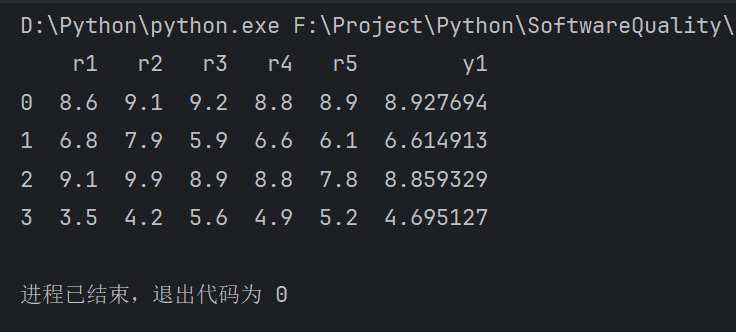
\includegraphics[width=0.45\textwidth]{img6/result1.png}
\end{figure}

\subsubsection{模型二}

以下为模型二的公式:
\[
y = \left( \sum_{i=1}^{n} \omega_i x_i^{-\rho_y} \right)^{-\frac{1}{\rho_y}}, \quad 1 \leq i \leq n, \quad 1 \leq x_i \leq 10.
\]

这与上一次作业中的形式也有一些相近,我们同样先进行 DataFrame 的构造:

由于 PPT 中有 $y_1$ 和 $y_2$ 的示例结果,我们可以先试着跑一个例子:

\begin{lstlisting} [language = Python, title = { 构造示例参数 }]
  test_data = {
      'x1': [8, 8, 6, 6, 9, 9, 3, 3],
      'x2': [9, 9, 7, 7, 10, 10, 4, 4],
      'x3': [10, 10, 5, 5, 9, 9, 5, 5],
      'x4': [8, 8, 6, 6, 8, 8, 4, 4],
      'rho_y': [0.10, 0.20, 0.10, 0.20, 0.10, 0.20, 0.10, 0.20]
  }
  test_weights = np.array([0.25, 0.20, 0.25, 0.30])
  df = pd.DataFrame(test_data)
\end{lstlisting}

\begin{lstlisting} [language = Python, title = { 计算 $y_2$ 的值 }]
  def calculate_y2(row):
    x_values = np.array([row['x1'], row['x2'], row['x3'], row['x4']])
    rho_y = row['rho_y']
    summation = np.sum(test_weights * (x_values ** -rho_y))
    y2 = summation ** (-1 / rho_y)
    return y2
\end{lstlisting}

\begin{lstlisting} [language = Python]
  def main():
    df['y2'] = df.apply(calculate_y2, axis=1)
    print(df)

  if __name__ == "__main__":
    main()
\end{lstlisting}

运行结果如下所示:

\begin{figure}[H]
  \centering
  \begin{subfigure}[b]{0.4\textwidth}
    \centering
    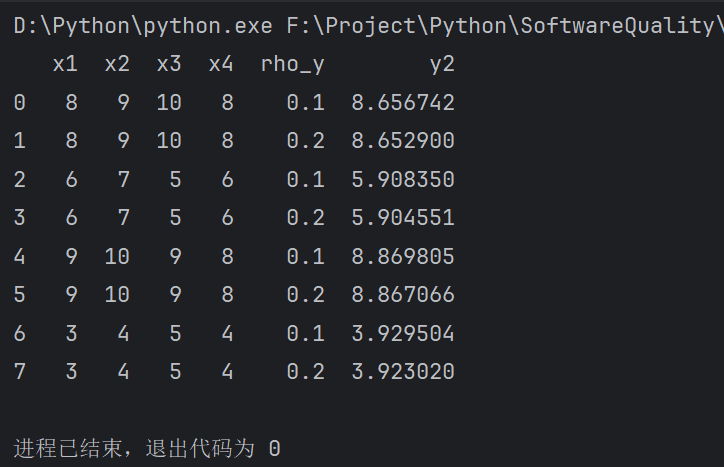
\includegraphics[width=\textwidth]{img6/resulttest.png}
    \caption{示例输出结果}
  \end{subfigure}
  \hspace{0.1\textwidth}
  \begin{subfigure}[b]{0.4\textwidth}
    \centering
    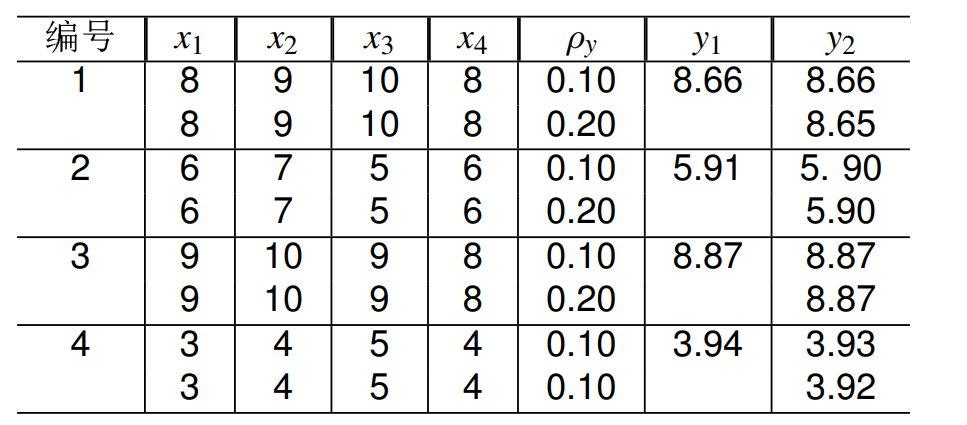
\includegraphics[width=\textwidth]{img6/contrast.png}
    \caption{PPT 上的示例结果对比}
  \end{subfigure}
  \caption{输出结果和 PPT 对比}
\end{figure}

可以发现,该代码成功计算了 $y_2$ 的值,与 PPT 中的示例结果基本一致。

\textbf{【Notice】:PPT 编号2 上 $\rho_y = 0.10$ 时,$y_2$ 的值应约为 5.91,而非 5.90}

接下来我们只需要把数据换成新的题目中的即可。

\begin{lstlisting} [language = Python]
  weights = np.array([0.15, 0.20, 0.20, 0.25, 0.20])
  data = {
    'x1': [8.6, 8.6, 6.8, 6.8, 9.1, 9.1, 3.5, 3.5],
    'x2': [9.1, 9.1, 7.9, 7.9, 9.9, 9.9, 4.2, 4.2],
    'x3': [9.2, 9.2, 5.9, 5.9, 8.9, 8.9, 5.6, 5.6],
    'x4': [8.8, 8.8, 6.6, 6.6, 8.8, 8.8, 4.9, 4.9],
    'x5': [8.9, 9.9, 6.1, 6.1, 7.8, 7.8, 5.2, 5.2],
    'rho_y': [0.01, 0.55, 0.01, 0.55, 0.01, 0.55, 0.01, 0.55]
  }
  df = pd.DataFrame(data)
\end{lstlisting}

后续只需要把对应的地方替换掉即可(test\_data 改为 data,test\_weights 改为 weights,注意还有 $x_5$ 的添加)

完整可运行代码如下所示:

\begin{lstlisting} [language = Python, title = { 计算 $y_2$ 的值 }]
  import numpy as np
  import pandas as pd
  
  weights = np.array([0.15, 0.20, 0.20, 0.25, 0.20])
  data = {
      'x1': [8.6, 8.6, 6.8, 6.8, 9.1, 9.1, 3.5, 3.5],
      'x2': [9.1, 9.1, 7.9, 7.9, 9.9, 9.9, 4.2, 4.2],
      'x3': [9.2, 9.2, 5.9, 5.9, 8.9, 8.9, 5.6, 5.6],
      'x4': [8.8, 8.8, 6.6, 6.6, 8.8, 8.8, 4.9, 4.9],
      'x5': [8.9, 9.9, 6.1, 6.1, 7.8, 7.8, 5.2, 5.2],
      'rho_y': [0.01, 0.55, 0.01, 0.55, 0.01, 0.55, 0.01, 0.55]
  }

  df = pd.DataFrame(data)

  def calculate_y2(row):
      x_values = np.array([row['x1'], row['x2'], row['x3'], row['x4'], row['x5']])
      rho_y = row['rho_y']
      summation = np.sum(weights * (x_values ** -rho_y))
      y2 = summation ** (-1 / rho_y)
      return y2

  def main():
      df['y2'] = df.apply(calculate_y2, axis=1)
      print(df)

  if __name__ == "__main__":
      main()
\end{lstlisting}

\subsubsection{模型二输出结果}
运行结果如下图所示:
\begin{figure}[H]
  \centering
  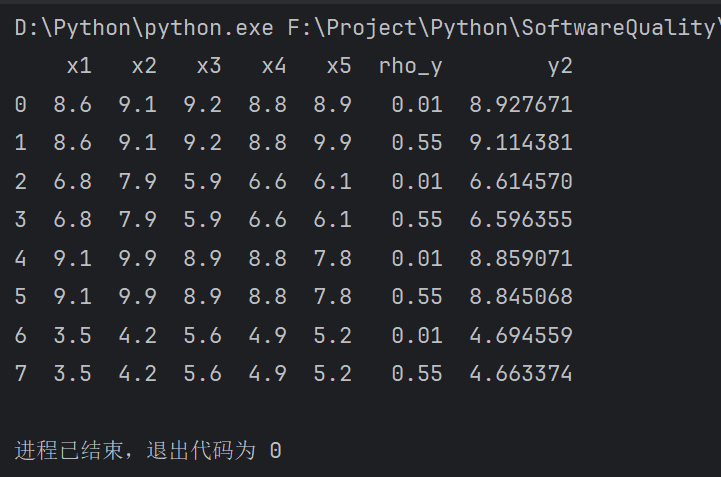
\includegraphics[width=0.4\textwidth]{img6/result2.png}
  \caption{模型二输出结果}
\end{figure}

\subsection{题目结果}

综上所述,对于模型一和模型二的计算,结果如下表所示:

\begin{table}[H]
  \centering
  \caption{作业三的数据}
  \begin{tabular}{|c|c|c|c|c|c|c|c|c|}
    \hline
    编号 & $x_1$ & $x_2$ & $x_3$ & $x_4$ & $x_5$ & $\rho_y$ & $y_1$ & $y_2$ \\
    \hline
    \multirow{2}{*}{1} & 8.6 & 9.1 & 9.2 & 8.8 & 8.9 & 0.01 & \multirow{2}{*}{8.927694} & 8.927671 \\
                       & 8.6 & 9.1 & 9.2 & 8.8 & 8.9 & 0.55 &                       & 9.114381 \\
    \hline
    \multirow{2}{*}{2} & 6.8 & 7.9 & 5.9 & 6.6 & 6.1 & 0.01 & \multirow{2}{*}{6.614913} & 6.614570 \\
                       & 6.8 & 7.9 & 5.9 & 6.6 & 6.1 & 0.55 &                       & 6.596355 \\
    \hline
    \multirow{2}{*}{3} & 9.1 & 9.9 & 8.9 & 8.8 & 7.8 & 0.01 & \multirow{2}{*}{8.859329} & 8.859071 \\
                       & 9.1 & 9.9 & 8.9 & 8.8 & 7.8 & 0.55 &                       & 8.845068 \\
    \hline
    \multirow{2}{*}{4} & 3.5 & 4.2 & 5.6 & 4.9 & 5.2 & 0.01 & \multirow{2}{*}{4.695127} & 4.694559 \\
                       & 3.5 & 4.2 & 5.6 & 4.9 & 5.2 & 0.55 &                       & 4.663374 \\
    \hline
  \end{tabular}
\end{table}

\section{作业四}

\subsection{题目内容}

设 \textbf{C919} 飞行控制软件有 \textbf{5} 个可信属性:实时性、可靠性、可生存性、可维护性、功能性(其含义见第 4 讲第 \textbf{3.2} 节),其正互反判断矩阵 \(\mathbf{A}\) 为
\[
\mathbf{A} = 
\begin{bmatrix}
    1 & 1/2 & 3 & 2 & 1/2 \\
    2 & 1 & 2 & 3 & 2 \\
    1/3 & 1/2 & 1 & 2 & 1/3 \\
    1/2 & 1/3 & 1/2 & 1 & 2 \\
    2 & 1/2 & 3 & 1/2 & 1 \\
\end{bmatrix}
\]

分别使用右特征向量法 \textbf{EV}、对数最小二乘法 \textbf{LLSM}、卡方最小二乘法 \textbf{CSM} 求出权重向量 \(\mathbf{W}^{EV}\)、\(\mathbf{W}^{LLSM}\)、\(\mathbf{W}^{CSM}\),在此基础上使用 “强度” 方法求出最优的权重向量。

\subsection{题目分析}

需要完整解答这道题,看来得列出四五段代码:

\subsubsection{右特征向量法 \textbf{EV}}
实在没有使用过 Python 处理矩阵,但显然 Numpy 中的 Array 也可以胜任这个角色。

关于特征值和特征向量的代码,我参考了网上的资料:

\textbf{numpy求特征值特征向量:}\href{https://blog.51cto.com/u_16099238/7589035}{\underline{https://blog.51cto.com/u\_16099238/7589035}}

\begin{lstlisting} [language = Python, title = { 右特征向量法 }]
  # 相似地,我们可以使用 PPT Test 中的示例先作为测试数据
  A = np.array([
    [1, 2, 4, 2, 2],
    [1/2, 1, 2, 1, 1/2],
    [1/4, 1/2, 1, 1/2, 2],
    [1/2, 1, 2, 1, 2],
    [1/2, 2, 1/2, 1/2, 1]
])

  def calculate_ev_weights(matrix):
    eigenvalues, eigenvectors = np.linalg.eig(matrix) # 返回值为元组,第一个元素为特征值,第二个元素为特征向量
    max_index = np.argmax(eigenvalues) # 取最大特征值对应的特征向量
    weights = eigenvectors[:, max_index].real
    # 归一化
    return weights / np.sum(weights)

  weights_ev = calculate_ev_weights(A)
\end{lstlisting}

测试效果良好,与PPT中的EA保持一致(0.3524, 0.1622, 0.1300, 0.2041, 0.1513):

\begin{figure}[H]
  \centering
  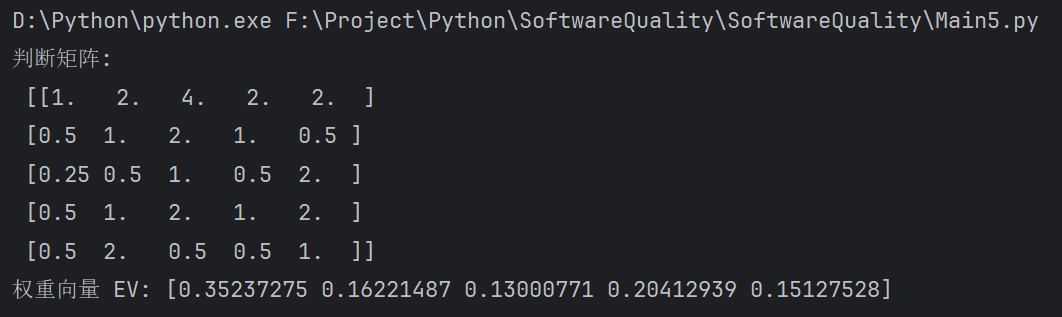
\includegraphics[width=0.6\textwidth]{img6/EVtest.png}
  \caption{右特征向量法权重向量}
\end{figure}

\subsubsection{对数最小二乘法 \textbf{LLSM}}

\begin{lstlisting} [language = Python, title = { 对数最小二乘法 }]
  def calculate_llsm_weights(matrix):
    numerator = np.prod(matrix, axis=1) ** (1 / matrix.shape[0])   # 分子 = 每行的乘积 × 开维度数次方
    denominator =  np.sum(numerator)   # 分母 = 每行的分子相加
    return numerator / denominator   # 归一化

  weights_llsm = calculate_llsm_weights(A)
  print("权重向量 W^LLSM:", weights_llsm)
\end{lstlisting}

测试效果良好,与PPT中的LLSM保持一致(0.3679, 0.1601, 0.1213, 0.2113, 0.1394):

\begin{figure}[H]
  \centering
  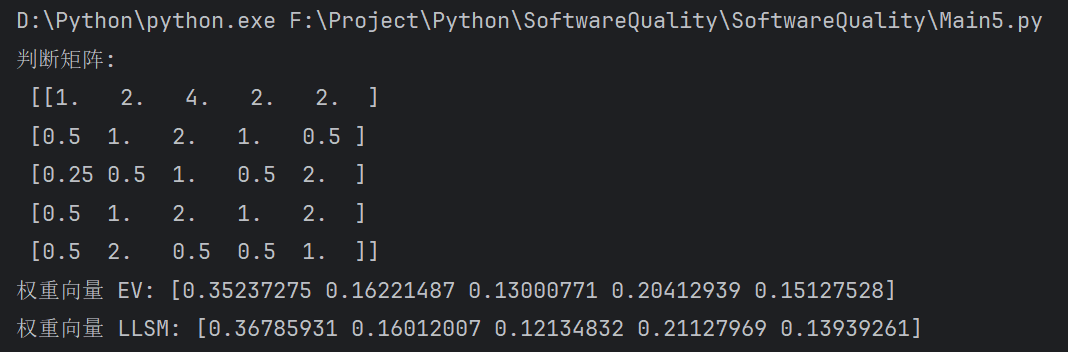
\includegraphics[width=0.6\textwidth]{img6/LLSMtest.png}
  \caption{对数最小二乘法权重向量}
\end{figure}

\subsubsection{卡方最小二乘法 \textbf{CSM}}

进入管理工程学报官网:\href{https://www.glgu.cbpt.cnki.net/WKG/WebPublication/wkTextContent.aspx?colType=4&yt=1994&st=01}{\underline{【管理工程学报】}}

知网检索:\href{https://kns.cnki.net/kcms2/article/abstract?v=pTDtInUJxYxjLD-7s1Jr5y1UuhV5yh60BdrEVEATp-rpr_LPiTYW74uV-MNF2f0Lr_QQDIvIRH5f-yqgGhgHumdqhClTNQyFcb65NEN6wwlrWuB-p4QMNaZegyN3DbXkOGmBu33PW1VPaiz8nddOdvkcMid0j-5daXosKJTzHSxUVCOpVL__ow==&uniplatform=NZKPT&language=CHS}{\underline{知网链接}}

查阅文献,与 PPT 中的内容相似:

\begin{figure}[H]
  \centering
  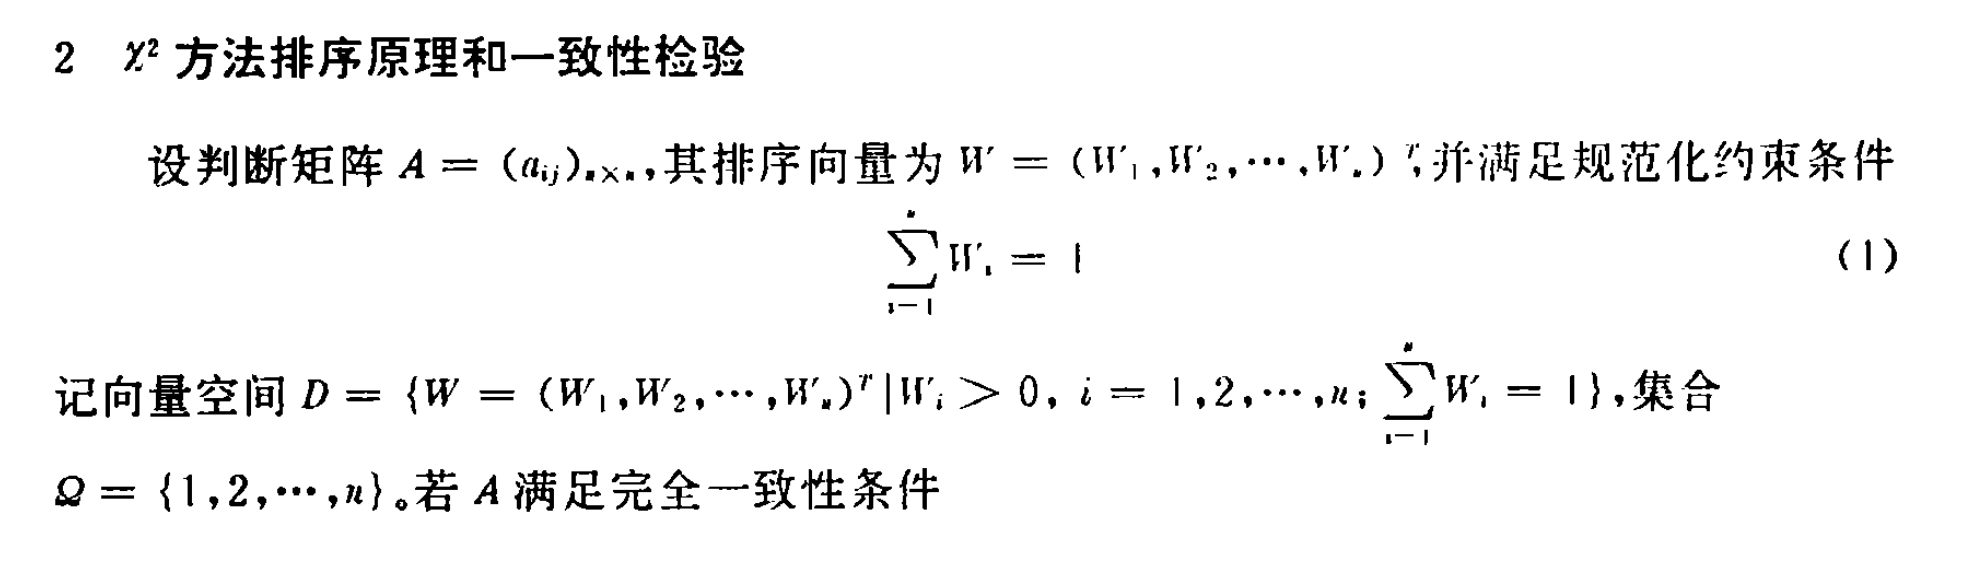
\includegraphics[width=0.6\textwidth]{img6/CSM.png}
  \caption{文献资料}
\end{figure}

其他的内容都是一些证明相关的,真正的算法精髓应该在于这里:

\begin{figure}[H]
  \centering
  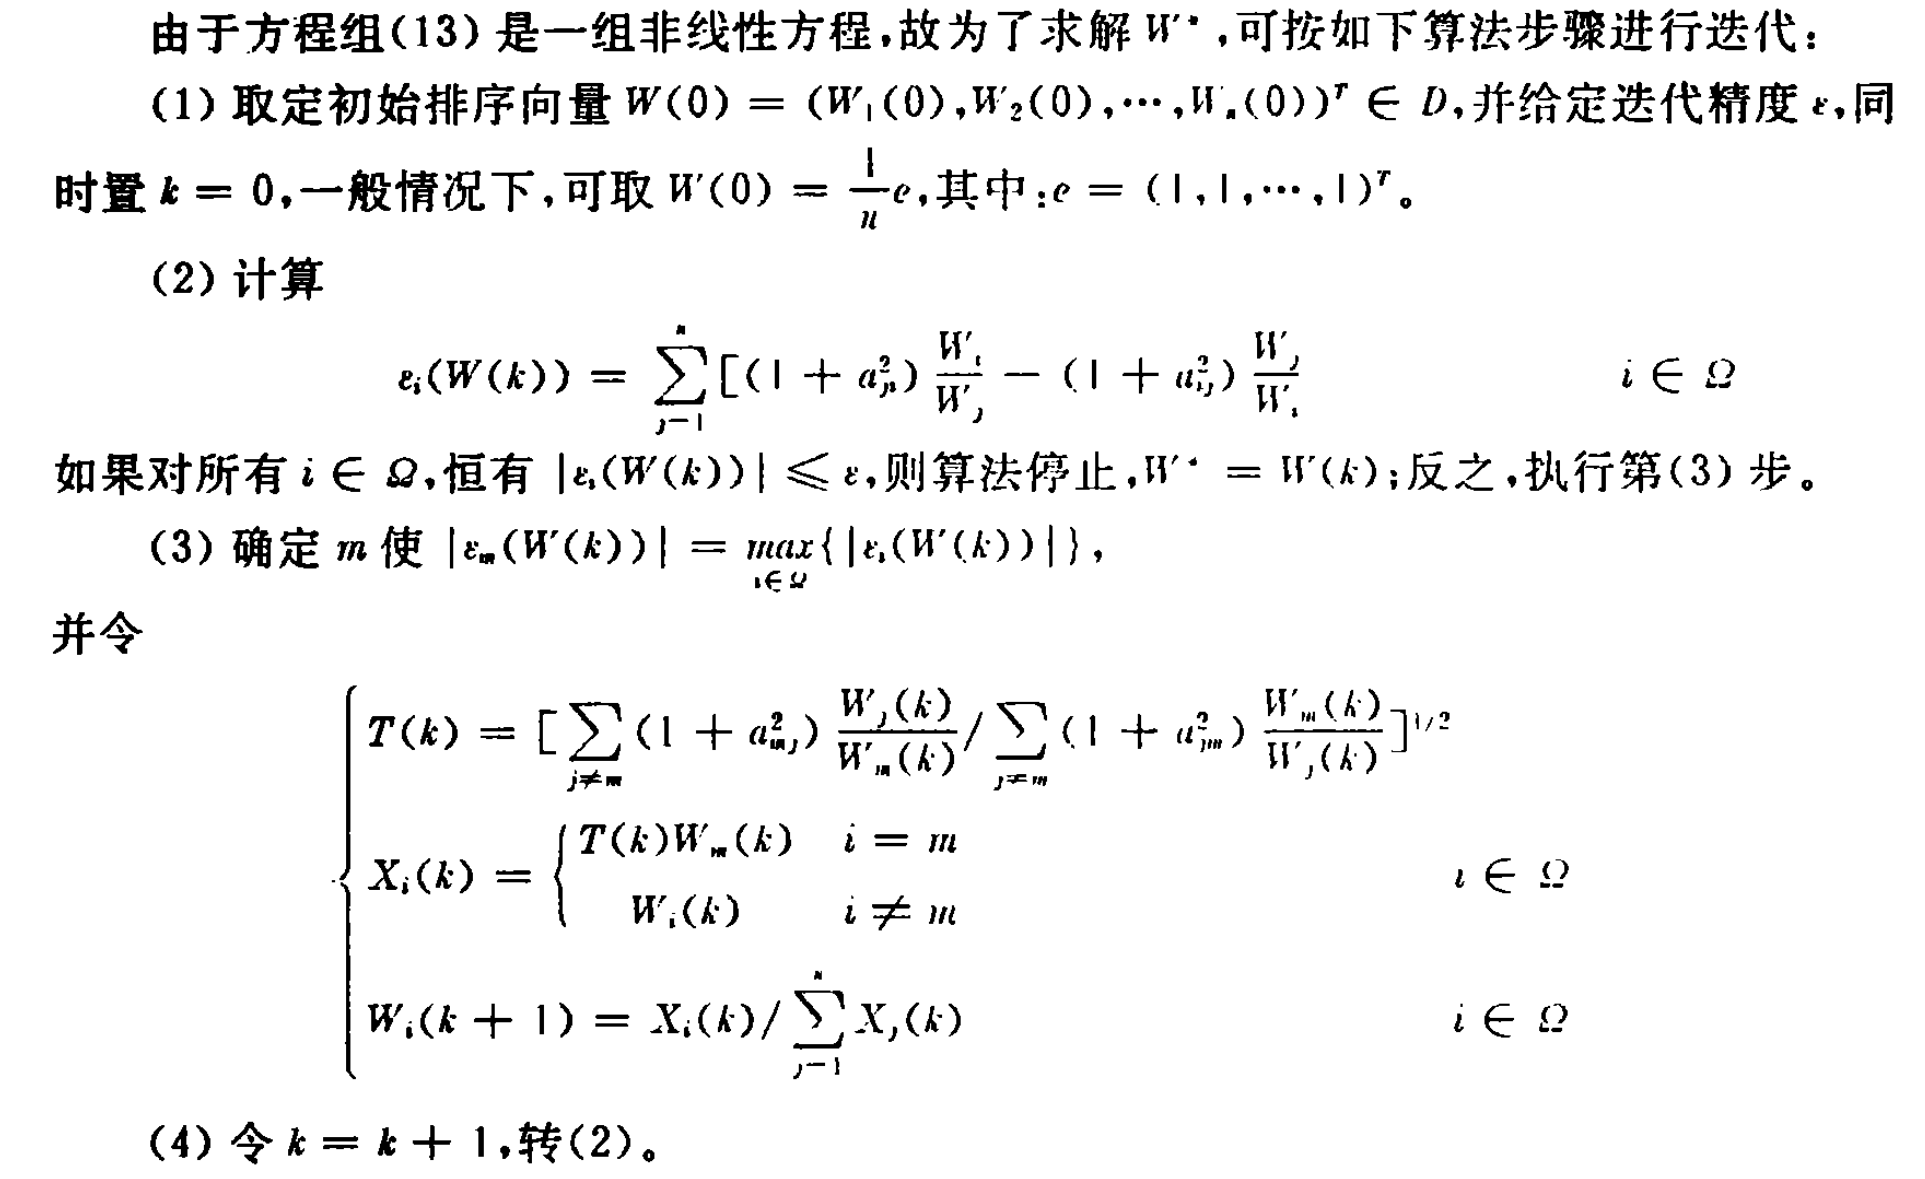
\includegraphics[width=0.6\textwidth]{img6/CSM2.png}
  \caption{迭代算法}
\end{figure}

复刻代码:

\begin{lstlisting} [language = Python, title = { 卡方最小二乘法 }]
  def calculate_csm_ppt():
  n = 5 # 方针阶数
  a = []
  print("输入方阵:")
  for i in range(0, n):
      row = list(map(float, input().split()))
      a.append(row)
  # 步骤 (1)
  epsilon = 1e-10
  w = [1 / n for i in range(0, n)] # 初始解
  while True:
      # 步骤 (2)
      m = None
      max_val = None
      for i in range(0, n):
          val = 0
          for j in range(0, n):
              val += (1 + a[j][i] * a[j][i]) * (w[i] / w[j]) - (1 + a[i][j] * a[i][j]) * (w[j] / w[i])
          val = abs(val)
          if max_val == None or val > max_val:
              max_val = val
              m = i
      if max_val != epsilon:
          break
      # 步骤(3)
      up = 0
      bottom = 0
      for j in range(0, n):
          if j != m:
              up += (1 + a[m][j] * a[m][j]) * (w[j] / w[m])
              bottom += (1 + a[j][m] * a[j][m]) * (w[m] / w[j])

      T = pow(up / bottom, 1 / 2)
      X = w
      X[m] *= T
      sum_X = sum(X)
      for i in range(0, n):
          w[i] = X[i] / sum_X
  return w
\end{lstlisting}

第一次运行时,该矩阵的输出为:[0.2, 0.2, 0.2, 0.2, 0.2] 并不符合预期。
为什么看起来全部都是初始解,而没有发生迭代呢?我猜测应该和判断结束的条件有关系,于是查看代码:

\begin{figure} [H]
  \centering
  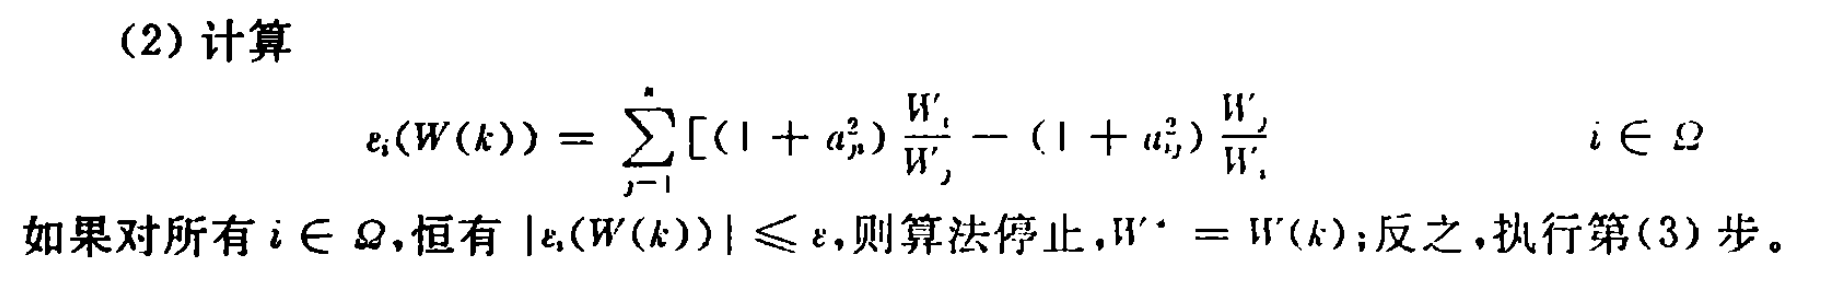
\includegraphics[width=0.6\textwidth]{img6/CSM3.png}
  \caption{结束条件}
\end{figure}

而在PPT给出的代码中,出现了感叹号和问号,是这里把我误导了:

\begin{figure} [H]
  \centering
  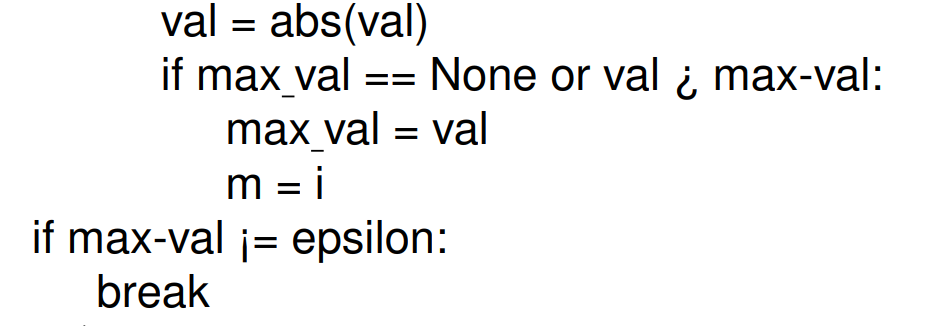
\includegraphics[width=0.3\textwidth]{img6/PPTCode.png}
  \caption{PPT代码}
\end{figure}

那么,根据文献内容,只要将 \texttt{max\_val != epsilon} 改为 \texttt{max\_val <= epsilon} 即可。

代码运行成功,与 PPT 完全一致(0.3767, 0.1546, 0.1186, 0.2121, 0.1379)

\begin{figure}[H]
  \centering
  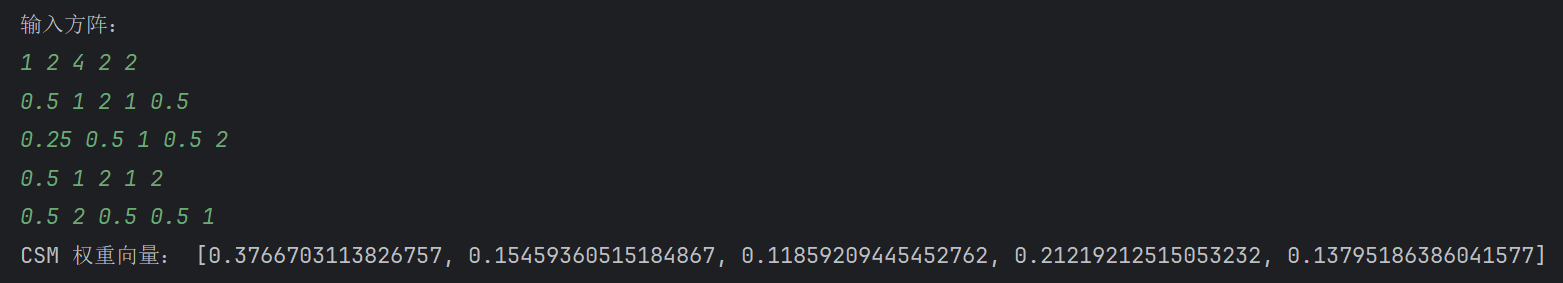
\includegraphics[width=0.8\textwidth]{img6/CSMtest.png}
  \caption{卡方最小二乘法权重向量计算结果}
\end{figure}

接下来,算法步骤明晰,不妨改写为使用 Numpy 来实现:

\begin{lstlisting} [language = Python, title = { 卡方最小二乘法 }]
  def calculate_csm_weights(matrix: np.array, epsilon: float, max_iterations: int) -> np.ndarray:
    '''计算 CSM,传入: matrix, precision, maximum iterations'''
    n = matrix.shape[0]
    # 初始化初始解
    W = np.ones(n) / n

    for k in range(max_iterations):
        e = np.zeros(n)
        for i in range(n):
            e[i] = np.sum([(1 + matrix[j, i] ** 2) * (W[i] / W[j]) - (1 + matrix[i, j] ** 2) * (W[j] / W[i])
                           for j in range(n) if j != i])

        max_e = np.max(np.abs(e))
        if max_e <= epsilon: # 若精度已到达,那么停止迭代
            print(f"在迭代次数为 {k} 次时收敛")
            break

        m = np.argmax(np.abs(e)) # 查找最大无差的索引

        # 计算 T(k)
        up = np.sum([(1 + matrix[m, j] ** 2) * (W[j] / W[m]) for j in range(n) if j != m])
        bottom = np.sum([(1 + matrix[j, m] ** 2) * (W[m] / W[j]) for j in range(n) if j != m])
        T = np.sqrt(up / bottom)

        # 更新矩阵向量,归一化
        X = W.copy()
        X[m] *= T
        W = X / np.sum(X)

    return W
\end{lstlisting}

测试结果与 PPT 一致:(0.3767, 0.1546, 0.1186, 0.2121, 0.1379)

\begin{figure}[H]
  \centering
  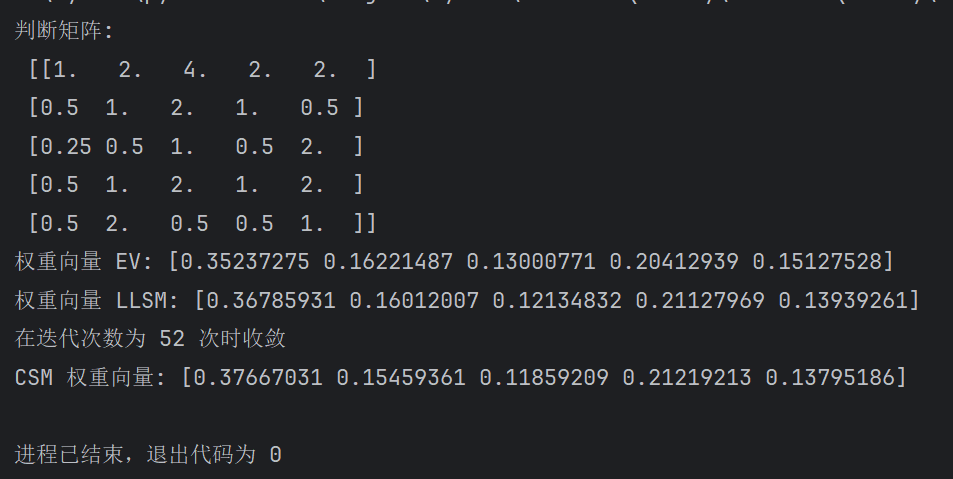
\includegraphics[width=0.5\textwidth]{img6/CSMtest2.png}
  \caption{卡方最小二乘法权重向量计算结果}
\end{figure}

\subsubsection{作业四三种权重向量的结果}
将数据修改为作业四中的矩阵,运行结果如下:

\begin{figure}[H]
  \centering
  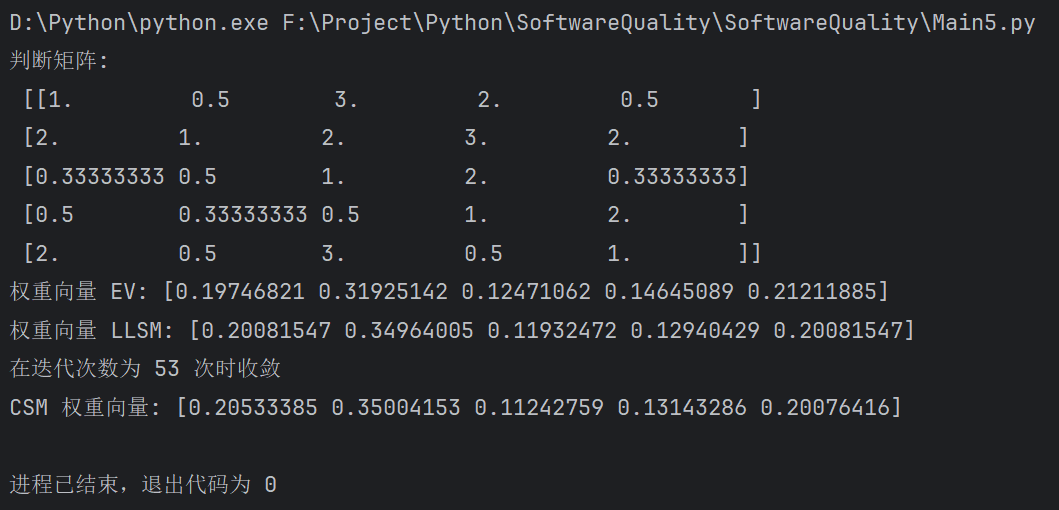
\includegraphics[width=0.5\textwidth]{img6/Homework4.png}
  \caption{卡方最小二乘法权重向量计算结果}
\end{figure}

\subsubsection{计算 TD 值}

对于任意给定的正互反判断矩阵,不同的优先级方法会得到不同的权重向量。
为了评价这些权重向量的质量,用两种评价标准:“程度”(strengths)和“方向”(directions)。

作业四要求使用 strengths 标准来衡量:

\begin{itemize}
  \item 使用“程度”评价准则来评估结果:
  \[
  TD^{(k)} = \sum_{i=1}^n \sum_{j=1}^n \left| a_{ij} - \frac{w_i^{(k)}}{w_j^{(k)}} \right|, \quad k = 1,2,3
  \]
  \item 比较不同方法计算出的 \( TD^{(1)}, TD^{(2)}, TD^{(3)} \) 值,选择最小 \( TD \) 所对应的权重向量为最优权重向量。
\end{itemize}

根据公式,可以写出计算 TD 值的代码:

\begin{lstlisting} [language = Python, title = { 计算 TD 值 }]
  def calculate_td(matrix: np.array, weight_vector: np.ndarray) -> float:
    n = len(weight_vector)
    td = 0.0
    for i in range(n):
        for j in range(n):
            td += abs(matrix[i, j] - (weight_vector[i] / weight_vector[j]))
    return td
\end{lstlisting}

相似地,我们先输入 PPT 中的示例,查看是否正确:

\begin{lstlisting} [language = Python, title = { 示例权重向量 }]
# PPT 中的权重向量
w1 = np.array([0.3524, 0.1622, 0.1300, 0.2041, 0.1513])
w2 = np.array([0.3679, 0.1601, 0.1213, 0.2113, 0.1394])
w3 = np.array([0.3767, 0.1546, 0.1186, 0.2121, 0.1379])

TD_EV = calculate_td(A, w1)
TD_LLSM = calculate_td(A, w2)
TD_CSM = calculate_td(A, w3)

print("TD EV:", TD_EV)
print("TD LLSM:", TD_LLSM)
print("TD CSM:", TD_CSM)

td_values = {"EV": TD_EV, "LLSM": TD_LLSM, "CSM": TD_CSM}
min_method = min(td_values, key=td_values.get)
print(f"最小的 TD 值为 {td_values[min_method]},选 {min_method} 计算的权重向量为可信属性的权重向量。")
\end{lstlisting}

输出结果如下:

\begin{figure} [H]
  \centering
  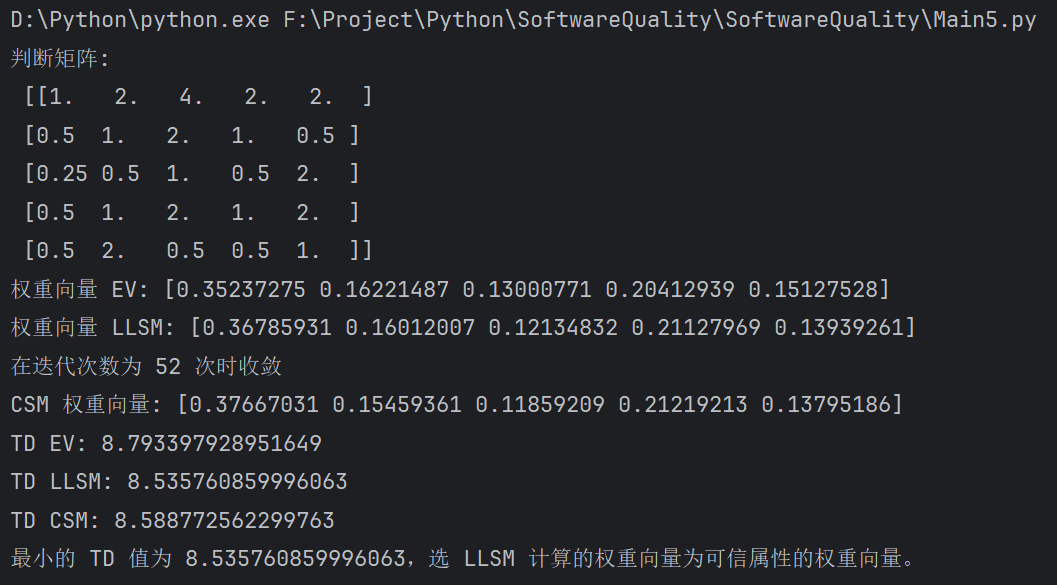
\includegraphics[width=0.5\textwidth]{img6/TDExample.png}
  \caption{TD 值示例计算结果}
\end{figure}

\subsection{题目结果}

将代码中的权重向量改为我们刚刚计算过后的结果,即整道题的答案如下所示:

\begin{figure} [H]
  \centering
  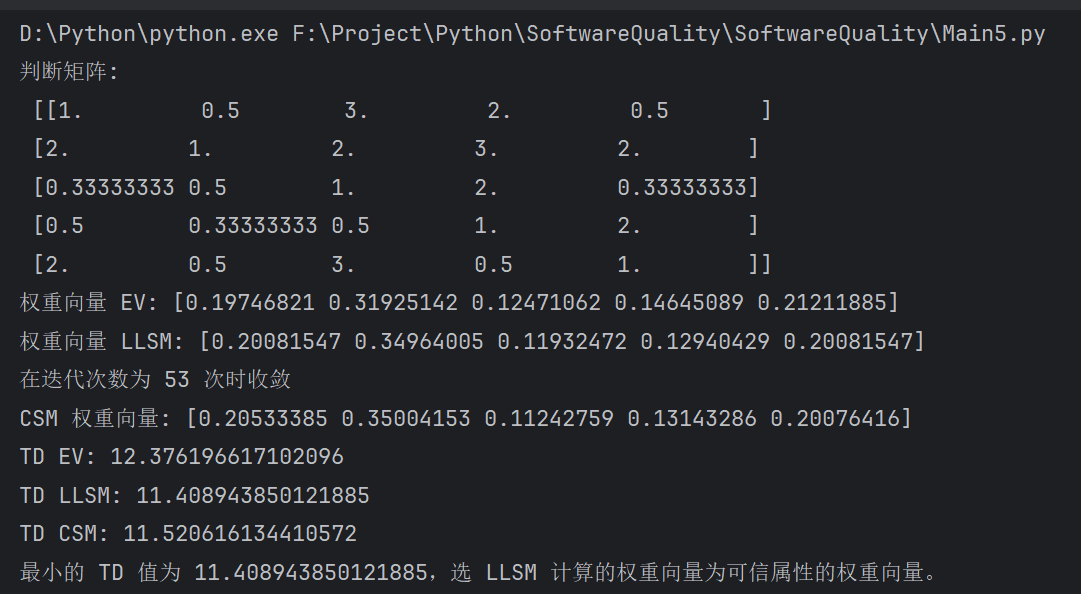
\includegraphics[width=0.5\textwidth]{img6/Homework4Result.png}
  \caption{作业四结果}
\end{figure}

最终结果如下所示:

\begin{ans}{作业四}{作业四}
  \textbf{正互反判断矩阵}:
  \[
  A = 
  \begin{bmatrix}
  1 & \frac{1}{2} & 3 & 2 & \frac{1}{2} \\
  2 & 1 & 2 & 3 & 2 \\
  \frac{1}{3} & \frac{1}{2} & 1 & 2 & \frac{1}{3} \\
  \frac{1}{2} & \frac{1}{3} & \frac{1}{2} & 1 & 2 \\
  2 & \frac{1}{2} & 3 & \frac{1}{2} & 1 \\
  \end{bmatrix}
  \]
\end{ans}
  
\bigskip
  
\begin{table}[H]
  \centering
  \begin{tabular}{c|c}
  \hline
  方法 & 权重向量 \\
  \hline
  EV   & (0.1975, 0.3193, 0.1247, 0.1465, 0.2121) \\ 
  LLSM & (0.2008, 0.3496, 0.1193, 0.1294, 0.2008) \\
  CSM  & (0.2053, 0.3500, 0.1124, 0.1314, 0.2008) \\
  \hline
  \end{tabular}
\end{table}

\begin{center}
三个权重向量的值分别为 $ TD^{EV} = 12.3762, TD^{LLSM} = 11.4089, TD^{CSM} = 11.5206 $。

最小的 TD 值为 11.408943850121885,选 LLSM 计算的权重向量为可信属性的权重向量。
\end{center}

\section{附录}

\subsection{参考文献}

\begin{itemize}
  \item 王应明, and 傅国伟. "判断矩阵排序的 $X^2$ 方法." 管理工程学报 8.1 (1994): 26-32.
  \item \textbf{numpy求特征值特征向量:}\underline{https://blog.51cto.com/u\_16099238/7589035}
\end{itemize}

\subsection{文件代码}

\begin{lstlisting} [language = Python, title = { Main.py }]
  # Code By Deralive (10235101526)
  # https://github.com/Shichien
  
  import numpy as np
  
  # 作业四矩阵
  A = np.array([
      [1, 1/2, 3, 2, 1/2],
      [2, 1, 2, 3, 2],
      [1/3, 1/2, 1, 2, 1/3],
      [1/2, 1/3, 1/2, 1, 2],
      [2, 1/2, 3, 1/2, 1]
  ])
  
  # # PPT 中的测试矩阵
  # A = np.array([
  #     [1, 2, 4, 2, 2],
  #     [1/2, 1, 2, 1, 1/2],
  #     [1/4, 1/2, 1, 1/2, 2],
  #     [1/2, 1, 2, 1, 2],
  #     [1/2, 2, 1/2, 1/2, 1]
  # ])
  
  def calculate_ev_weights(matrix):
      eigenvalues, eigenvectors = np.linalg.eig(matrix)  # 返回值为元组,第一个元素为特征值,第二个元素为特征向量
      max_index = np.argmax(eigenvalues)  # 取最大特征值对应的特征向量
      weights = eigenvectors[:, max_index].real
      # 归一化
      return weights / np.sum(weights)
  
  def calculate_llsm_weights(matrix):
      # 分子 = 每行的乘积 × 开维度数次方
      numerator = np.prod(matrix, axis=1) ** (1 / matrix.shape[0])
      # 分母 = 每行的分子相加
      denominator =  np.sum(numerator)
      # 归一化
      return numerator / denominator
  
  def calculate_csm_weights(matrix: np.array, epsilon: float, max_iterations: int) -> np.ndarray:
      '''计算 CSM,传入: matrix, precision, maximum iterations'''
      n = matrix.shape[0]
      # 初始化初始解
      W = np.ones(n) / n
  
      for k in range(max_iterations):
          e = np.zeros(n)
          for i in range(n):
              e[i] = np.sum([(1 + matrix[j, i] ** 2) * (W[i] / W[j]) - (1 + matrix[i, j] ** 2) * (W[j] / W[i])
                             for j in range(n) if j != i])
  
          max_e = np.max(np.abs(e))
          if max_e <= epsilon: # 若精度已到达,那么停止迭代
              print(f"在迭代次数为 {k} 次时收敛")
              break
  
          m = np.argmax(np.abs(e)) # 查找最大无差的索引
  
          # 计算 T(k)
          up = np.sum([(1 + matrix[m, j] ** 2) * (W[j] / W[m]) for j in range(n) if j != m])
          bottom = np.sum([(1 + matrix[j, m] ** 2) * (W[m] / W[j]) for j in range(n) if j != m])
          T = np.sqrt(up / bottom)
  
          # 更新矩阵向量,归一化
          X = W.copy()
          X[m] *= T
          W = X / np.sum(X)
  
      return W
  
  def calculate_csm_weights_ppt():
      n = 5 # 方针阶数
      a = []
      print("输入方阵:")
      for i in range(0, n):
          row = list(map(float, input().split()))
          a.append(row)
      # 步骤 (1)
      epsilon = 1e-10
      w = [1 / n for i in range(0, n)] # 初始解
      while True:
          # 步骤 (2)
          m = None
          max_val = None
          for i in range(0, n):
              val = 0
              for j in range(0, n):
                  val += (1 + a[j][i] * a[j][i]) * (w[i] / w[j]) - (1 + a[i][j] * a[i][j]) * (w[j] / w[i])
              val = abs(val)
              if max_val == None or val > max_val:
                  max_val = val
                  m = i
          if max_val <= epsilon:
              break
          # 步骤(3)
          up = 0
          bottom = 0
          for j in range(0, n):
              if j != m:
                  up += (1 + a[m][j] * a[m][j]) * (w[j] / w[m])
                  bottom += (1 + a[j][m] * a[j][m]) * (w[m] / w[j])
  
          T = pow(up / bottom, 1 / 2)
          X = w
          X[m] *= T
          sum_X = sum(X)
          for i in range(0, n):
              w[i] = X[i] / sum_X
      return w
  
  def calculate_td(matrix: np.array, weight_vector: np.ndarray) -> float:
      n = len(weight_vector)
      td = 0.0
      for i in range(n):
          for j in range(n):
              td += abs(matrix[i, j] - (weight_vector[i] / weight_vector[j]))
      return td
  
  weights_ev = calculate_ev_weights(A)
  print("判断矩阵:\n", A)
  print("权重向量 EV:", weights_ev)
  
  weights_llsm = calculate_llsm_weights(A)
  print("权重向量 LLSM:", weights_llsm)
  
  # weight_vec_tor_csm_ppt = calculate_csm_ppt()
  # print("CSM 权重向量:", weight_vec_tor_csm_ppt)
  
  weight_csm = calculate_csm_weights(A, 1e-10, 1000)
  print("CSM 权重向量:", weight_csm)
  
  # # PPT 中的权重向量
  # w1 = np.array([0.3524, 0.1622, 0.1300, 0.2041, 0.1513])
  # w2 = np.array([0.3679, 0.1601, 0.1213, 0.2113, 0.1394])
  # w3 = np.array([0.3767, 0.1546, 0.1186, 0.2121, 0.1379])
  
  # 新的权重向量
  w1 = np.array([0.1975, 0.3193, 0.1247, 0.1465, 0.2121])  # EV
  w2 = np.array([0.2008, 0.3496, 0.1193, 0.1294, 0.2008])  # LLSM
  w3 = np.array([0.2053, 0.3500, 0.1124, 0.1314, 0.2008])  # CSM
  
  TD_EV = calculate_td(A, w1)
  TD_LLSM = calculate_td(A, w2)
  TD_CSM = calculate_td(A, w3)
  
  print("TD EV:", TD_EV)
  print("TD LLSM:", TD_LLSM)
  print("TD CSM:", TD_CSM)
  
  td_values = {"EV": TD_EV, "LLSM": TD_LLSM, "CSM": TD_CSM}
  min_method = min(td_values, key=td_values.get)
  print(f"最小的 TD 值为 {td_values[min_method]},选 {min_method} 计算的权重向量为可信属性的权重向量。")  
\end{lstlisting}
\end{document}